%! TEX root = thesis_pres.tex

\section{Results}
\subsection{Small Dataset}
\label{sub:small_dataset}

\begin{frame}[t]{Test Description}
  \begin{itemize}
    \item Training set and testing set
      \begin{itemize}
        \item Initialize with training set
        \item Try to relocalize frames in testing set
      \end{itemize}
    \item Ground Truth Baseline 
      \begin{itemize}
        \item Use GT data to find optimal Place Finder
      \end{itemize}
    \item Performance showed histogram of translation error
  \end{itemize}


  \only<2>{
    \centering
    \includegraphics[width=0.5\linewidth]{large_dataset/CC_esm_dist.eps}
  }
  
\end{frame}



\begin{frame}[t]{Results small dataset}
  \begin{itemize}
    \item 10 images for training and 10 images for testing
    \item 237 world points
    \item 2 square meters area
  \end{itemize}
      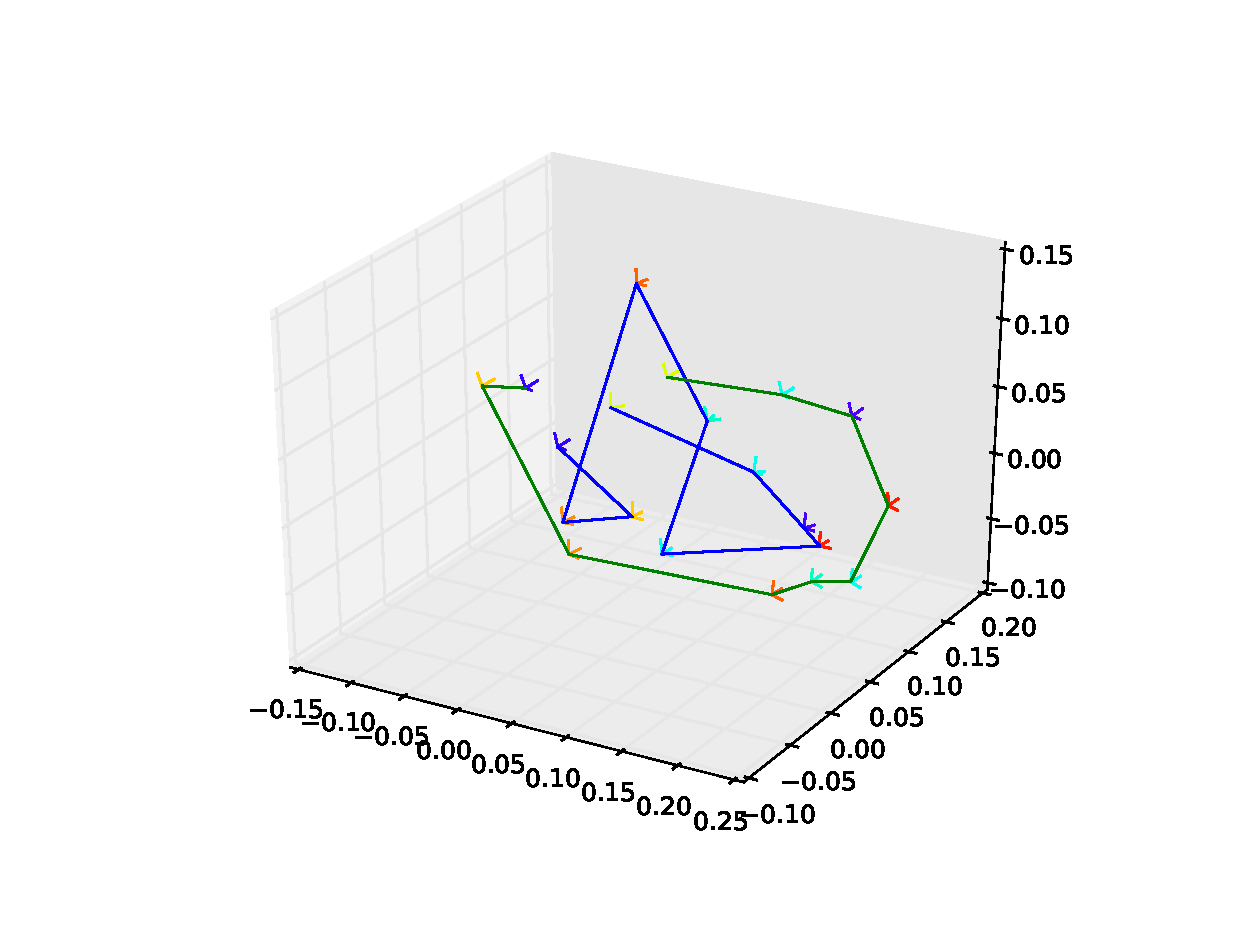
\includegraphics[width=0.5\linewidth]{small_dataset/desktop_2_train_test.eps}
      \includegraphics[width=0.5\linewidth]{small_dataset/image00654.png}
  
\end{frame}

\begin{frame}[t]{Results small dataset}
  %\setbeamerfont{caption}{size=\tiny}%{size=\tiny}
  \captionsetup[sub]{labelformat=empty,font=scriptsize,textfont=scriptsize,labelfont=scriptsize}
  \begin{figure}	
    \centering
    \begin{subfigure}[t]{0.2\linewidth}
      \centering
      \includegraphics[width=1\linewidth]{small_dataset/desktop_2_naive_empty_dist_1.png}
      \caption{Only GT mean error = 0.17}		
    \end{subfigure}
    \quad
    \begin{subfigure}[t]{0.2\linewidth}
      \centering
      \includegraphics[width=1\linewidth]{small_dataset/desktop_2_naive_esm_dist_1.png}
      \caption{GT and ESM mean error = 0.10}
    \end{subfigure}
    \quad
    \begin{subfigure}[t]{0.2\linewidth}
      \centering
      \includegraphics[width=1\linewidth]{small_dataset/desktop_2_naive_3pt_dist_1.eps}
      \caption{GT and P3P mean error = 0.02}
    \end{subfigure}
    \hfill\null
    \\
    \begin{subfigure}[t]{0.2\linewidth}
      \centering
      \includegraphics[width=1\linewidth]{small_dataset/desktop_2_CC_empty_dist_1.png}
      \caption{Only CC mean error = 0.19}
    \end{subfigure}
    \quad
    \begin{subfigure}[t]{0.2\linewidth}
      \centering
      \includegraphics[width=1\linewidth]{small_dataset/desktop_2_CC_esm_dist_1.eps}
      \caption{CC and ESM mean error = 0.15}
    \end{subfigure}
    \quad
    \begin{subfigure}[t]{0.2\linewidth}
      \centering
      \includegraphics[width=1\linewidth]{small_dataset/desktop_2_CC_3pt_dist_1.png}
      \caption{CC and P3P mean error = 0.11}
    \end{subfigure}
    \begin{subfigure}[t]{0.2\linewidth}
      \centering
      \includegraphics[width=1\linewidth]{small_dataset/desktop_2_ferns_60_12_dist_1.eps}
      \caption{\textit{ferns} mean error = 0.02}
    \end{subfigure}
    \hfill\null
    \caption{Translation error histograms}
  \end{figure}

\end{frame}



\begin{frame}[t]{Results small dataset}

  \captionsetup[sub]{labelformat=empty, font=small}
  \begin{figure}	
    \centering
    \begin{subfigure}[t]{.45\linewidth}
      \centering
      \includegraphics[width=\linewidth]{small_dataset/desktop_2_CC_3pt_path_1.png}
      \caption{Path found with CC and P3P}		
    \end{subfigure}
    \hfill
    \begin{subfigure}[t]{.45\linewidth}
      \centering
      \includegraphics[width=\linewidth]{small_dataset/desktop_2_ferns_60_12_path_1.eps}
      \caption{Path found with \textit{ferns}}		
    \end{subfigure}
  \end{figure}

\end{frame}

\subsection{Large Dataset}
\label{sub:large_dataset}


\begin{frame}[t]{Results large dataset}
  \begin{itemize}
    \item 84 images for training and 69 images for testing
    \item 1730 world points
    \item 7x3 meters area 
  \end{itemize}
      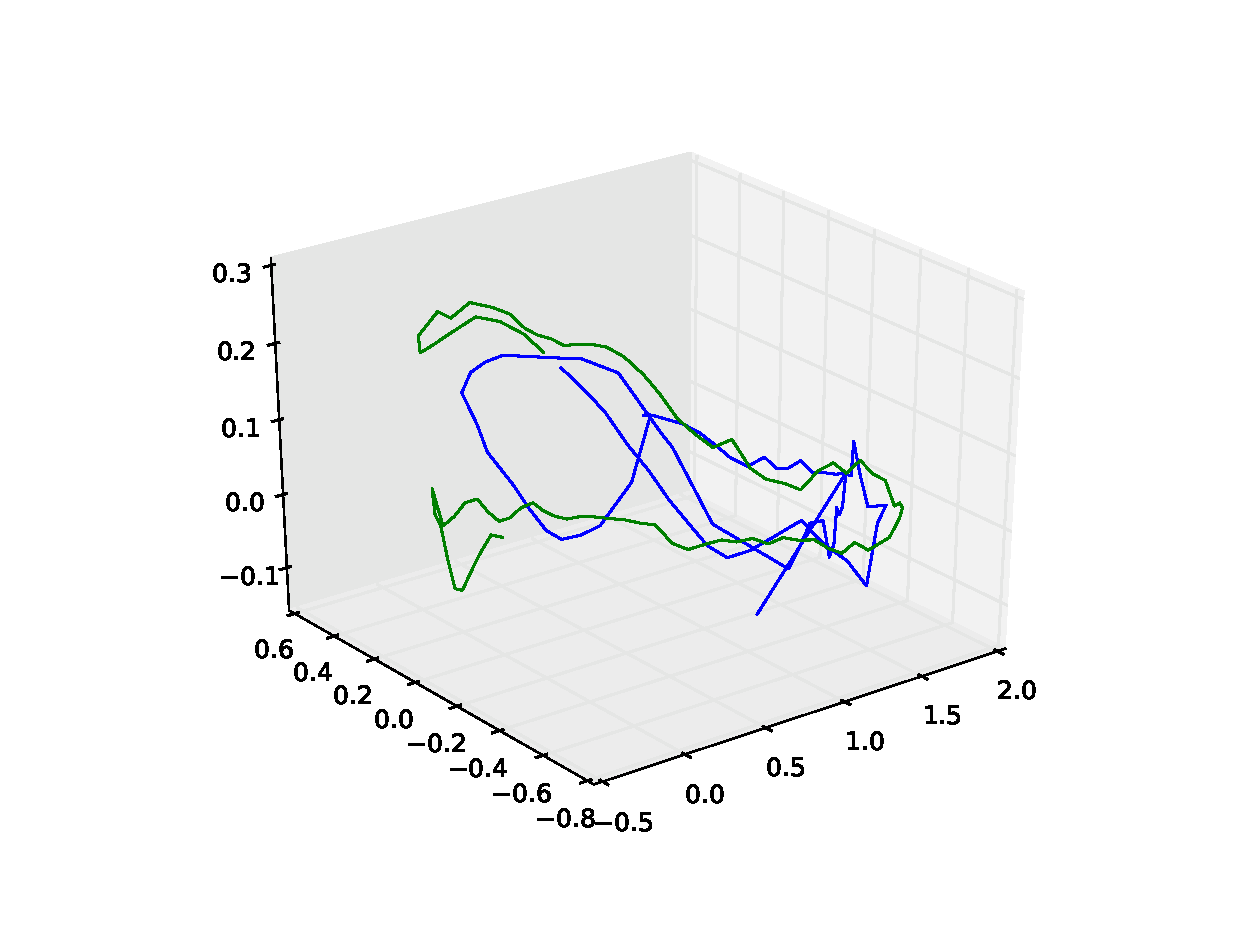
\includegraphics[width=0.5\linewidth]{large_dataset/test_train_path.eps}
      \includegraphics[width=0.5\linewidth]{large_dataset/image00778.png}
  
\end{frame}

\begin{frame}[t]{Results large dataset with \textit{ferns}}

  \captionsetup[sub]{labelformat=empty, font=small}
  \begin{figure}	
    \centering
    \begin{subfigure}[t]{.45\linewidth}
      \centering
        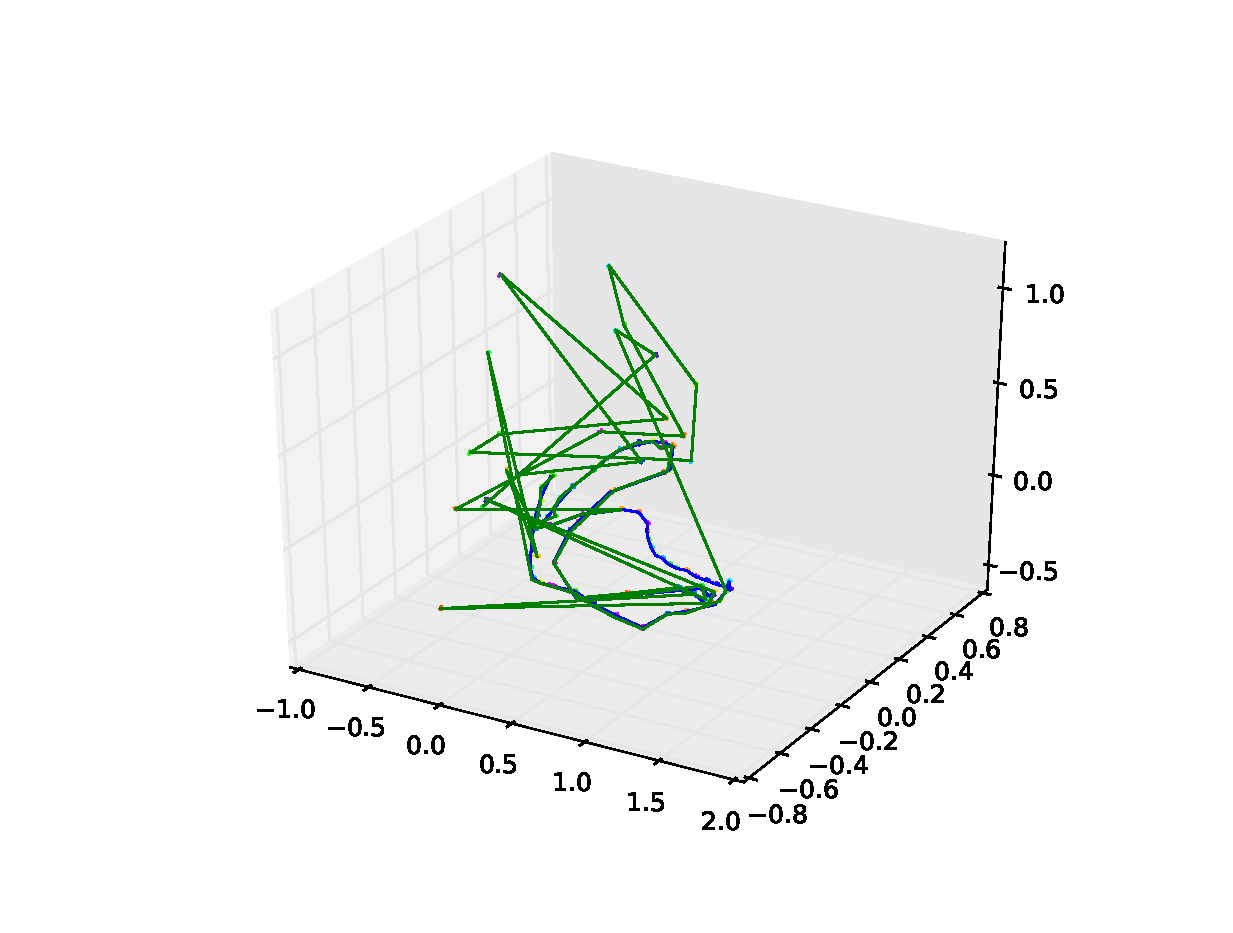
\includegraphics[width=\linewidth]{large_dataset/ferns_100_path.eps}
      \caption{Path found with \textit{ferns}}		
    \end{subfigure}
    \hfill
    \begin{subfigure}[t]{.45\linewidth}
      \centering
      \includegraphics[width=\linewidth]{large_dataset/ferns_100_dist.eps}
      \caption{\textit{ferns} error histogram. 45/69}		
    \end{subfigure}
  \end{figure}

\end{frame}

\begin{frame}[t]{Timing}

  \begin{figure}[htpb]
    \centering
    \begin{bchart}[steps={0.2,0.4,0.6,0.8,1},max=1]
      \bcbar[label= CC and ESM]{0.0437}
      \bcbar[label=CC and P3P]{0.0647}
      \bcbar[label=ferns 237 classes]{0.128}
      \bcbar[label=ferns 1730 classes]{0.933}
    \end{bchart}
    \caption{Single relocalization execution time in seconds}
    \label{fig:exec_time}
  \end{figure}


  \begin{figure}[htpb]
    \centering
    \begin{bchart}[step=10, max=70]
      \bcbar[label=\quad 237 classes]{5.57}
      \bcbar[label=1730 classes]{63.11}
    \end{bchart}
    \caption{\textit{ferns} classifier training time in seconds}
    \label{fig:training_time}
  \end{figure}
\end{frame}
%\begin{frame}[t]{Naive \textit{Place Finder}}
%  This method uses GT data to find the closest frame.
%  \begin{figure}[!ht]
%    \subfloat[In blue GT. In green found poses]{%
%      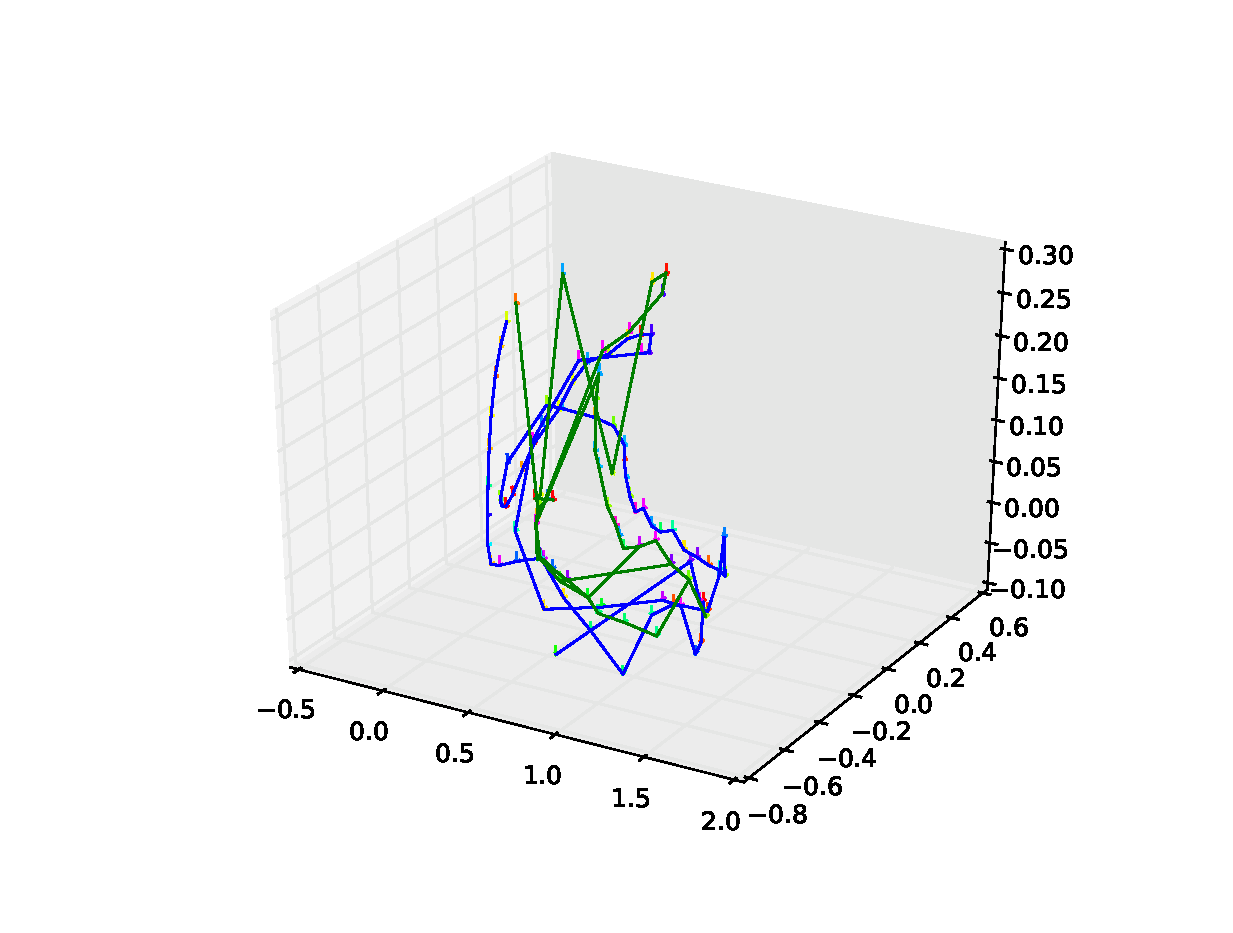
\includegraphics[width=0.47\linewidth]{large_dataset/naive_empty_path.eps}
%    }
%    \hfill
%    \subfloat[Error]{%
%      \includegraphics[width=0.47\linewidth]{large_dataset/naive_empty_dist.eps}
%    }
%  \end{figure}
%\end{frame}
%
%\begin{frame}[t]{CC \textit{Place Finder}}
%  \begin{figure}[!ht]
%    \only<1>{
%      \subfloat[In blue GT. In green found poses]{%
%        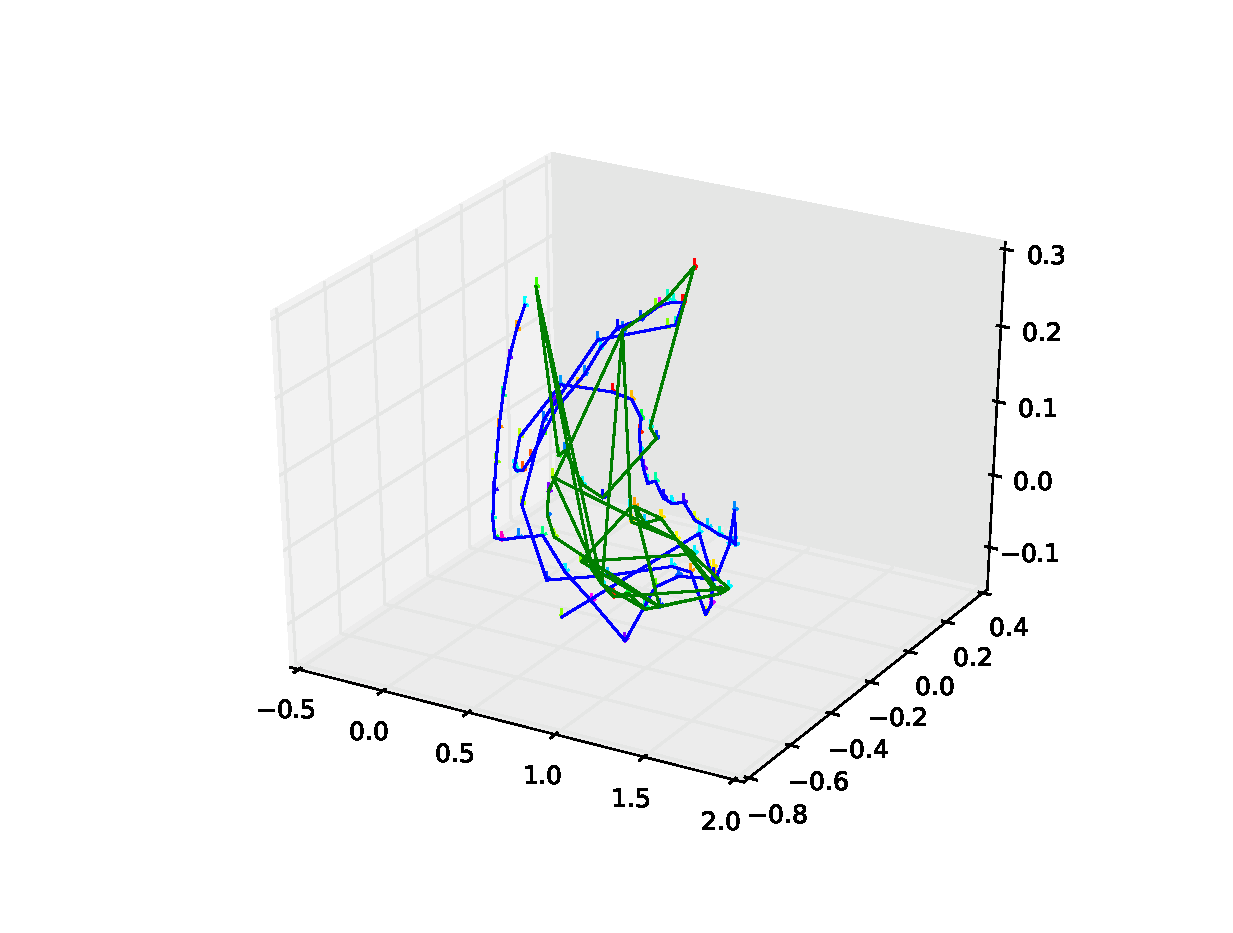
\includegraphics[width=0.47\linewidth]{large_dataset/CC_empty_path.eps}}
%    }
%      \only<2>{
%      \subfloat[Error with naive Pose Finder]{%
%        \includegraphics[width=0.47\linewidth]{large_dataset/naive_empty_dist.eps}}
%    }
%    \hfill
%    \subfloat[CC Error]{%
%      \includegraphics[width=0.47\linewidth]{large_dataset/CC_empty_dist.eps}
%    }
%  \end{figure}
%\end{frame}
%
%\begin{frame}[t]{ESM \textit{Real Pose Finder}}
%  \begin{figure}[!ht]
%    \only<1>{
%      \subfloat[In blue GT. In green found poses]{%
%        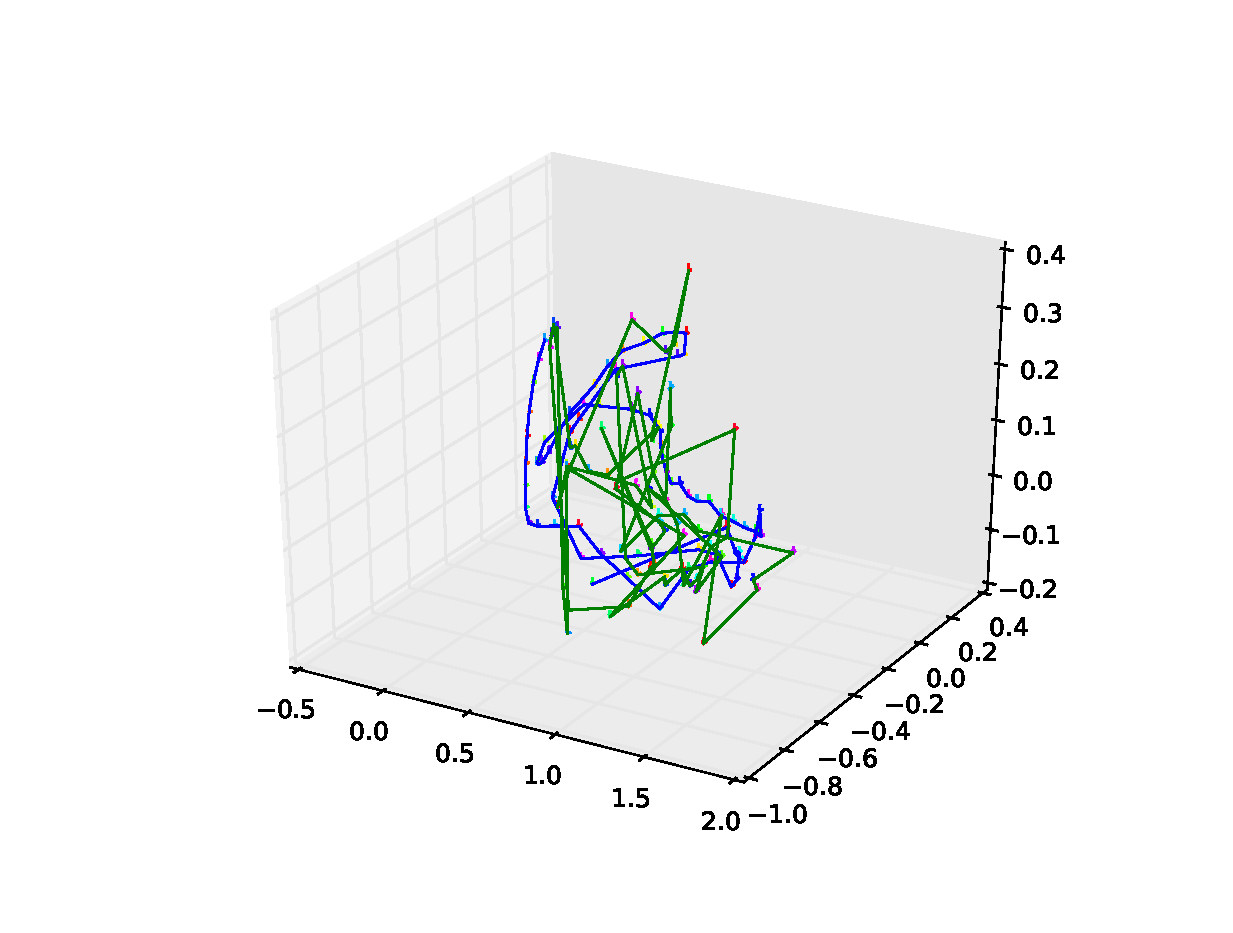
\includegraphics[width=0.47\linewidth]{large_dataset/CC_esm_path.eps}}
%    }
%    \only<2>{
%      \subfloat[Error CC]{%
%        \includegraphics[width=0.47\linewidth]{large_dataset/CC_empty_dist.eps}}
%    }
%    \only<3>{
%      \subfloat[Error with naive Pose Finder]{%
%        \includegraphics[width=0.47\linewidth]{large_dataset/naive_esm_dist.eps}}
%    }
%    \hfill
%    \subfloat[Error ESM]{%
%      \includegraphics[width=0.47\linewidth]{large_dataset/CC_esm_dist.eps}
%    }
%  \end{figure}
%\end{frame}
%
%\begin{frame}[t]{Three-point \textit{Real Pose Finder}}
%  \begin{figure}[!ht]
%    \only<1>{
%      \subfloat[In blue GT. In green found poses]{%
%        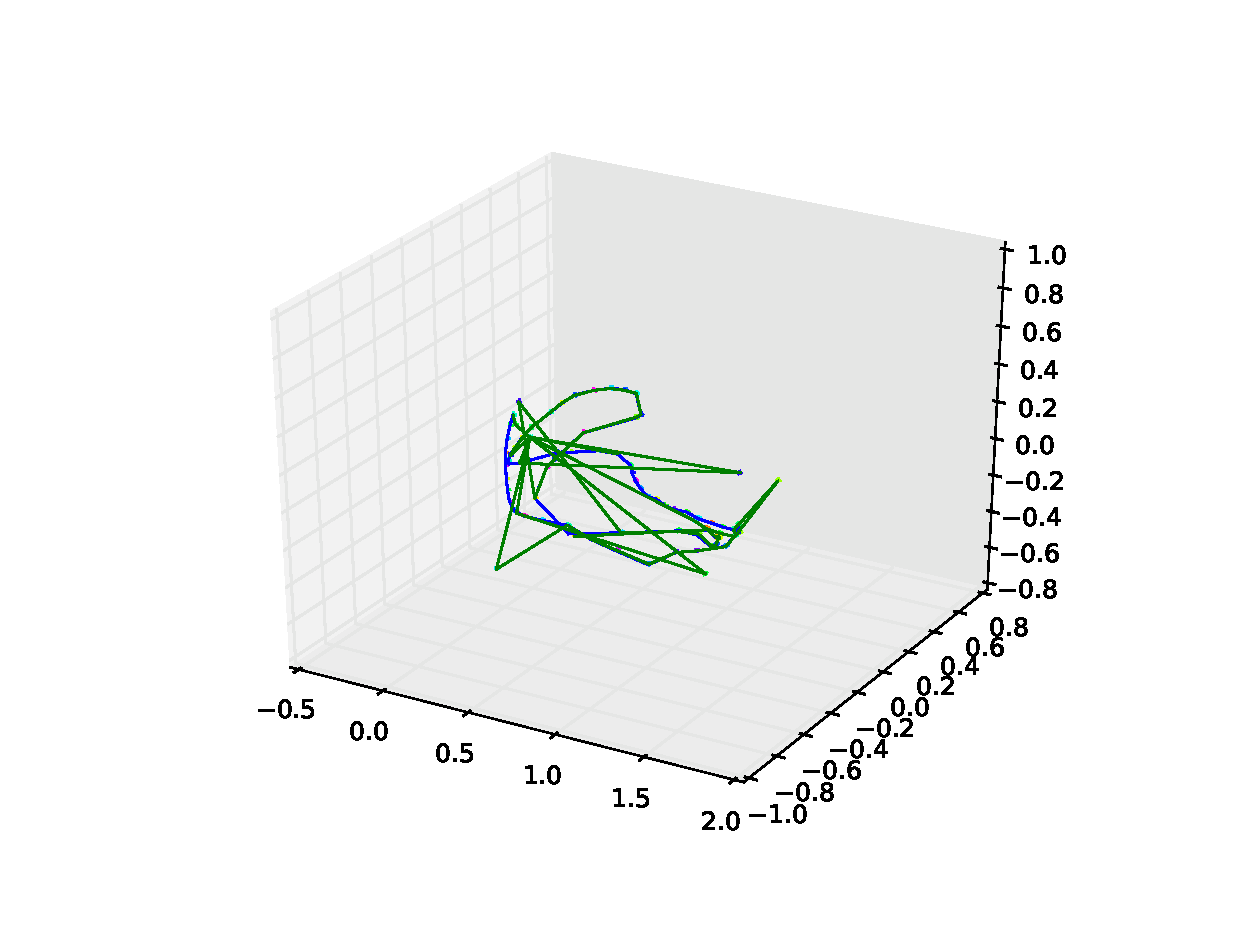
\includegraphics[width=0.47\linewidth]{large_dataset/CC_3pt_path.eps}}
%    }
%    \only<2>{
%      \subfloat[Error CC]{%
%        \includegraphics[width=0.47\linewidth]{large_dataset/CC_empty_dist.eps}}
%    }
%    \only<3>{
%      \subfloat[Error with naive Pose Finder]{%
%        \includegraphics[width=0.47\linewidth]{large_dataset/naive_3pt_dist.eps}}
%    }
%    \hfill
%    \subfloat[Error three-points]{%
%      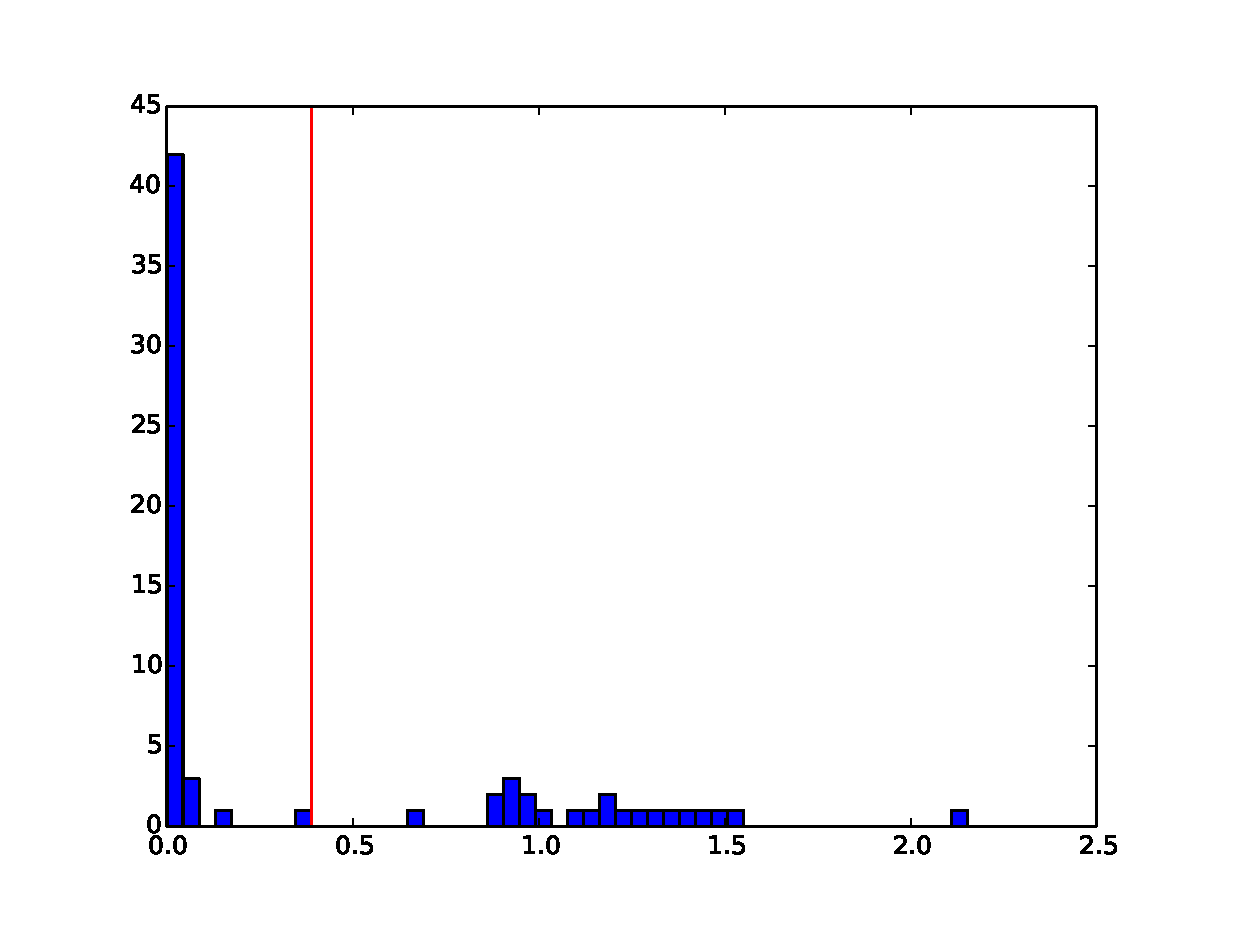
\includegraphics[width=0.47\linewidth]{large_dataset/CC_3pt_dist.eps}
%    }
%  \end{figure}
%\end{frame}
%
%\begin{frame}[t]{\textit{Ferns} Relocalizer}
%  \begin{figure}[!ht]
%    \only<1>{
%      \subfloat[In blue GT. In green found poses]{%
%        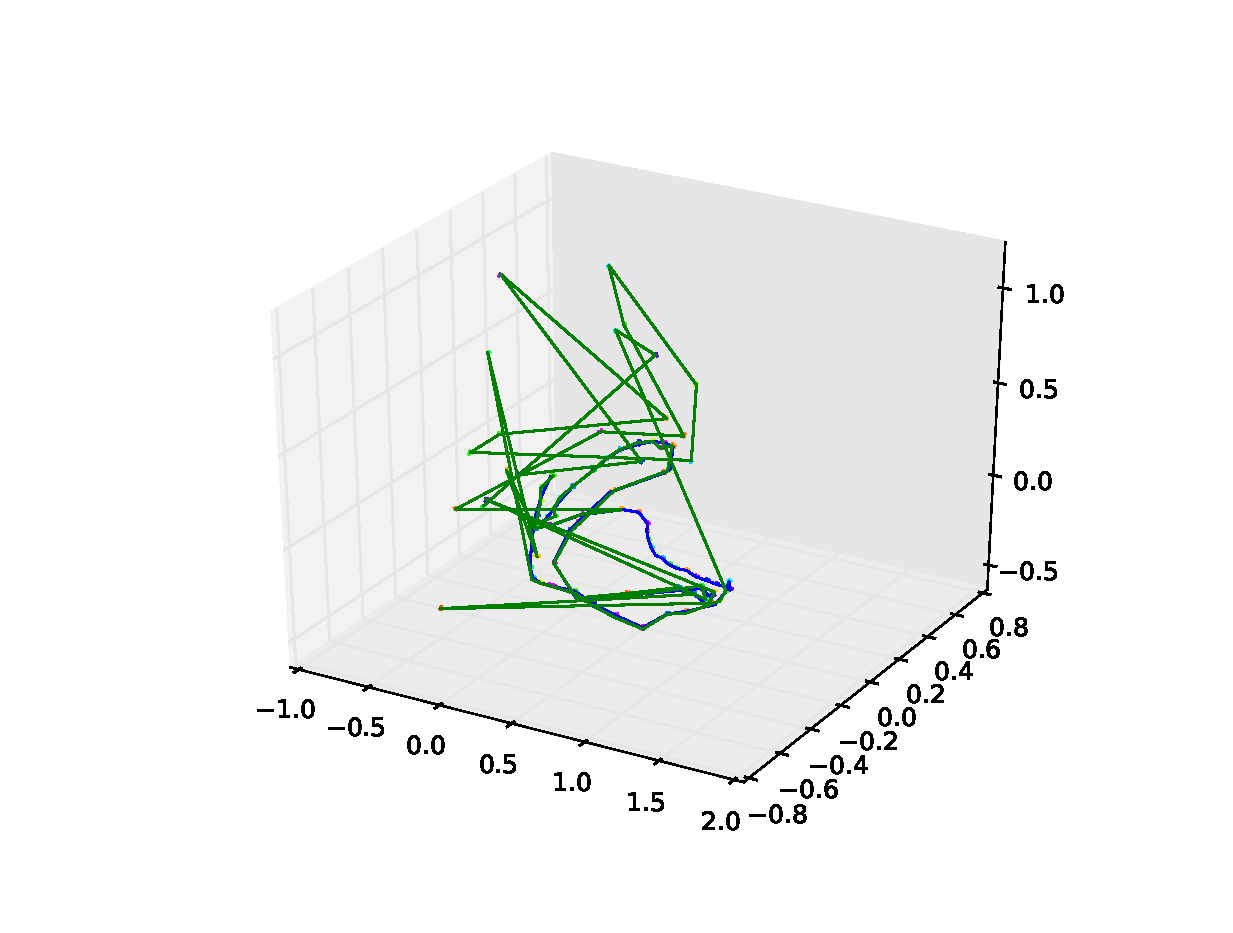
\includegraphics[width=0.47\linewidth]{large_dataset/ferns_100_path.eps}}
%    }
%    \only<2>{
%      \subfloat[Error three-points]{%
%        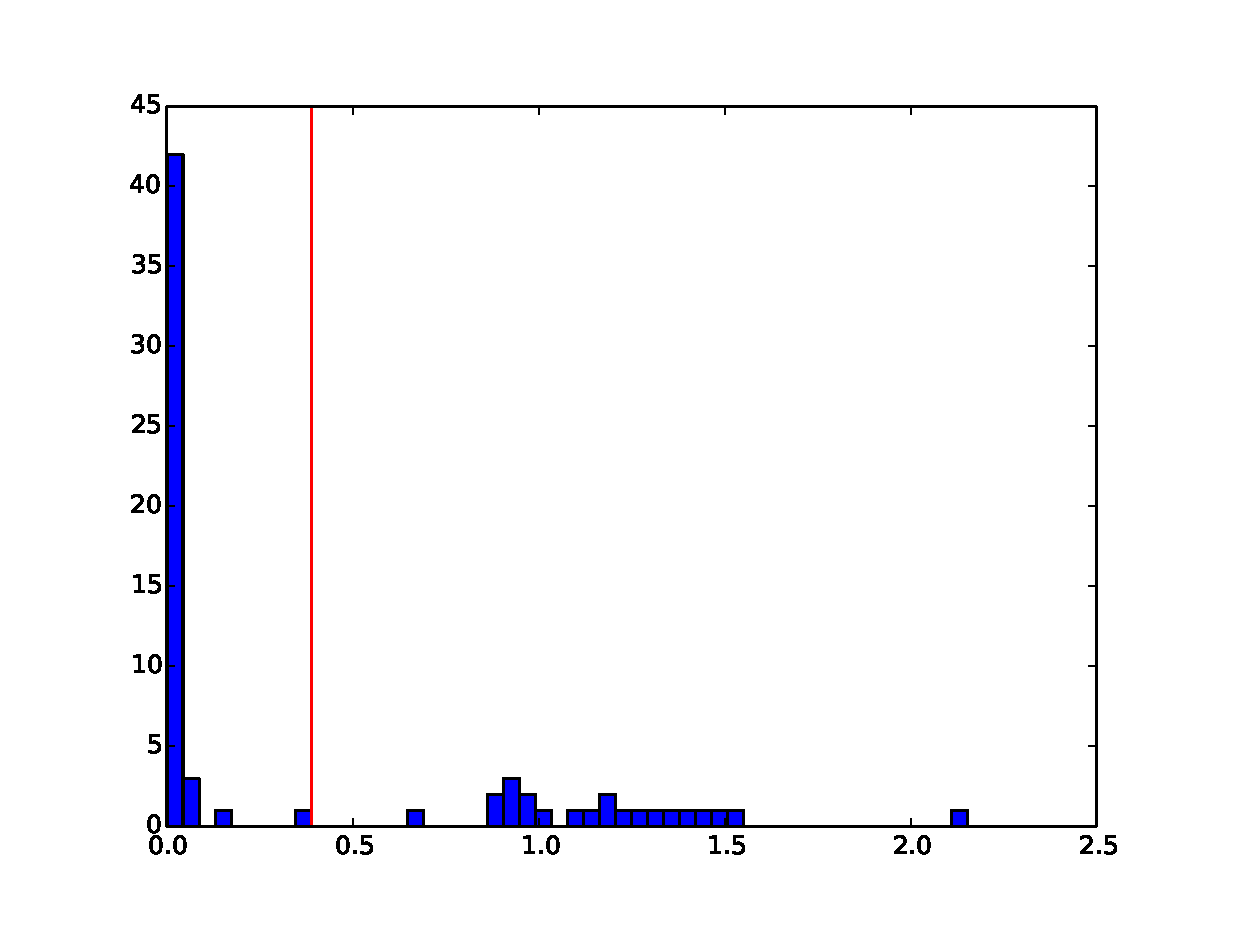
\includegraphics[width=0.47\linewidth]{large_dataset/CC_3pt_dist.eps}}
%    }
%    \hfill
%    \subfloat[Error \textit{ferns}]{%
%      \includegraphics[width=0.47\linewidth]{large_dataset/ferns_100_dist.eps}
%    }
%  \end{figure}
%\end{frame}

